% !Mode:: "TeX:UTF-8"
\documentclass{article}
% !Mode:: "TeX:UTF-8"
\usepackage[english]{babel}
\usepackage[UTF8]{ctex}
\usepackage{amsmath, amsthm, amssymb}

% Figure
\usepackage{graphicx}
\usepackage{float} %% H can fix the location
\usepackage{caption}
\usepackage[format=hang,singlelinecheck=0,font={sf,small},labelfont=bf]{subfig}
\usepackage[noabbrev]{cleveref}
\captionsetup[subfigure]{subrefformat=simple,labelformat=simple,listofformat=subsimple}
\renewcommand\thesubfigure{(\alph{subfigure})}

\usepackage{epstopdf} %% convert eps to pdf
\DeclareGraphicsExtensions{.eps,.mps,.pdf,.jpg,.png} %% bmp, gif not supported
\DeclareGraphicsRule{*}{eps}{*}{}
\graphicspath{{img/}{figure/}{../figure/}} %% fig directorys

%% \usepackage{pstricks} %% a set of macros that allow the inclusion of PostScript drawings directly inside TeX or LaTeX code
%% \usepackage{wrapfig} %% Wrapping text around figures

% Table
\usepackage{booktabs} %% allow the use of \toprule, \midrule, and \bottomrule
\usepackage{tabularx}
\usepackage{multirow}
\usepackage{colortbl}
\usepackage{longtable}
\usepackage{supertabular}

\usepackage[colorinlistoftodos]{todonotes}

% Geometry
\usepackage[paper=a4paper, top=1.5cm, bottom=1.5cm, left=1cm, right=1cm]{geometry}
%% \usepackage[paper=a4paper, top=2.54cm, bottom=2.54cm, left=3.18cm, right=3.18cm]{geometry} %% ms word
%% \usepackage[top=0.1cm, bottom=0.1cm, left=0.1cm, right=0.1cm, paperwidth=9cm, paperheight=11.7cm]{geometry} %% kindle

% Code
%% \usepackage{alltt} %% \textbf can be used in alltt, but not in verbatim

\usepackage{listings}
\lstset{
    backgroundcolor=\color{white},
    columns=flexible,
    breakatwhitespace=false,
    breaklines=true,
    captionpos=tt,
    frame=single, %% Frame: show a box around, possible values are: none|leftline|topline|bottomline|lines|single|shadowbox
    numbers=left, %% possible values are: left, right, none
    numbersep=5pt,
    showspaces=false,
    showstringspaces=false,
    showtabs=false,
    stepnumber=1, %% interval of lines to display the line number
    rulecolor=\color{black},
    tabsize=2,
    texcl=true,
    title=\lstname,
    escapeinside={\%*}{*)},
    extendedchars=false,
    mathescape=true,
    xleftmargin=3em,
    xrightmargin=3em,
    numberstyle=\color{gray},
    keywordstyle=\color{blue},
    commentstyle=\color{green},
    stringstyle=\color{red},
}

% Reference
%% \bibliographystyle{plain} % reference style

% Color
\usepackage[colorlinks, linkcolor=blue, anchorcolor=red, citecolor=green, CJKbookmarks=true]{hyperref}
\usepackage{color}
\def\red#1{\textcolor[rgb]{1.00,0.00,0.00}{#1}}
\newcommand\warning[1]{\red{#1}}

% Other
%% \usepackage{fixltx2e} %% for use of \textsubscript
%% \usepackage{dirtree}  %% directory structure, like the result of command tree in bash shell

   %导入需要用到的package
% !Mode:: "TeX:UTF-8"
%+++++++++++++++++++++++++++++++++++article+++++++++++++++++++++++++++++++++
%customize the numbering of equation, to make it like section-subsection-equation style, for example,1-2-3
\makeatletter\@addtoreset{equation}{subsection}\makeatother
\renewcommand\theequation{%
\thepart\arabic{section}%
-\thepart\arabic{subsection}%
-\thepart\arabic{equation}%
}
%theorem
\newtheorem{definition}{D\'efintion} %% 整篇文章的全局编号
\newtheorem*{thmwn}{Thm} %% without numbers
\newtheorem{theorem}{Th\'eor\`eme}[section] %% 从属于section编号
\newtheorem{corollary}{Corollary}[theorem] %% 从属于theorem编号
\newtheorem{lemma}{Lemma}
\newtheorem{proposition}{Proposition}[section]
\newtheorem{example}{Example}
\newtheorem*{attention}{Attention}
\newtheorem*{note}{Note}
\newtheorem*{remark}{Remark}
\newtheorem{question}{Question}[section]
\newtheorem{problem}{Problem}
\newtheorem{fact}{Fact}

   %导入需要用到的package
\begin{document}
\title{Introduction to algorithm \\Eric's Notes}
\author{Eric}
\maketitle
\newpage
\tableofcontents
\newpage

\section{课程简介及算法分析}
\subsection{Insertion sort}
Pseudocode
\begin{verbatim}
INSERTION-SORT(A)
1 for j ← 2 to length[A]  #1是第一个元素
2 	do key ← A[j] //将将要插入的数据保存下来
3 	//Insert A[j] into the sorted sequence A[1 _ j - 1].
4	 i ← j - 1
5	 while i > 0 and A[i] > key
6		 do A[i + 1] ← A[i]
7		 i ← i - 1
8	 A[i + 1] ← key
\end{verbatim}
\begin{figure}[htbp]
  \centering
  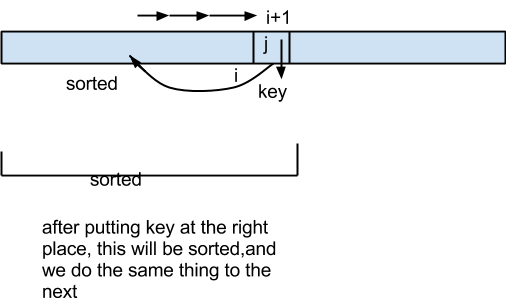
\includegraphics[scale = 0.7]{sort_insertion}\\
  \caption{Insertion sort}\label{fig.sort.insertion}
\end{figure}

ex:
\begin{verbatim}
8 2 4 9 3 6
2 8 4 9 3 6 // 2 goes before 8
2 4 8 9 3 6 // 4 goes before 8
2 4 8 9 3 6 // 9 stays there
2 3 4 8 9 6 // 3 goes before 4
2 3 4 6 8 9 // 6 goes before 8
\end{verbatim}

\begin{figure}[htbp]
  \centering
  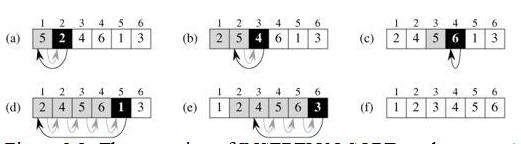
\includegraphics[scale = 0.7]{sort_insertion_example}\\
  \caption{Insertion sort}\label{fig.sort.insertion.example}
\end{figure}

python code
\begin{verbatim}
def insertionSort(L):
	#in place algorithem, 升序
	for j in range(1,len(L)):
		#将将要排序的数据保存下来, 开始对第j 个元素进行排序
		key=L[j]
		i=j-1
		#找到存放key的位置
		while i >= 0 and L[i]>key:
			L[i+1]=L[i] ## 将大数往后移动
			i=i-1
		##循环结束,说明L[i] <= key,所以key应该放在i+1处
		L[i+1]=key
	return L
\end{verbatim}

running time\\
1 already sorted: 最理想情况\\
2 reverse sorted: 最差情况

we want upper bounds 上界

kinds of analysis\\
worst-case $T(n)=max$ time of any input of size n\\
average-case $T(n)=expected time$期望时间\\
(need assumption of statistical  distribution of inputs)\\
best-case (bogus假象)

BIG IDEA: \textbf{asymptotic analysis渐进分析}\\
not the the exact running time of an algorithm\\
the order of growth of the running time

the insertion sort analysis\\
worst-case: input reverse sorted
$$T(n)=\sum_{j=2}^{j=n} \theta(j)=\theta(n^2) \eqnote{算术级数arithmetic series}$$

\subsection{Merge sort}
算法\\
T(n) merge sort A[1...n]\\
$\theta(1)$	1 if n=1, done\\
$2*\theta(n/2)$	2 Recursively sort A[1...upper(n/2)] and A[upper(n/2)+1...n]    向上取整\\
$\theta(n)$	3 merge 2 sorted  list

Merge\\
Where is the smallest element of any two lists that are already sorted?\\
It is in one of two places, the head of the first list or the head of the second list

\textbf{Key subroutine Merge}
\begin{verbatim}
2 7 13 20
1 9 11 12
\end{verbatim}
在两个list head中,1最小,所以1是n个元素中最小的,排在最终的list的第一个位置,现在总list和两个子list成为:
\begin{verbatim}
1
2 7 13 20
9 11 12
\end{verbatim}
然后在比较两个子list 中head位置那个更小,把它放在总list的第二个位置
\begin{verbatim}
1 2
7 13 20
9 11 12
\end{verbatim}
一直这么继续下去,
这里的每一步都是固定数目的操作,和每一步中的数组的尺寸无关,每一步总,我们只关注两个head,并挑出最小的,再把数组指针推进一位,所以我知道当前的标头在哪里.
所以,对于总数为n的输入,时间是$\theta(n)$的
所以把两个list遍历和排序的时间是$\theta(n)$,有时我们称之为线性时间

merge sort的例子
\begin{figure}[htbp]
  \centering
  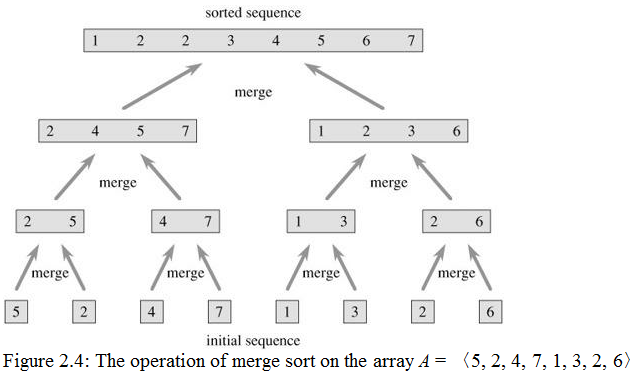
\includegraphics[scale = 0.7]{sort_merge_example}\\
  \caption{Merge sort example}\label{fig.sort.merge.example}
\end{figure}

时间复杂度
$$
T(n) =
\left\{
  \begin{array}{ll}
	\theta(1) \si n=1 \\
	2*T(n/2) + \theta(n) \si n>1
  \end{array}
\right.
$$

\subsection{Recursion tree}
一直做下去,得到,每一行的和都为$cn$,数的深度为$\lg n$,树的level是$\lg n+1$,最后一层的叶节点有$n$个,每一个都是$\theta(1)$

\begin{figure}[htbp]
  \centering
  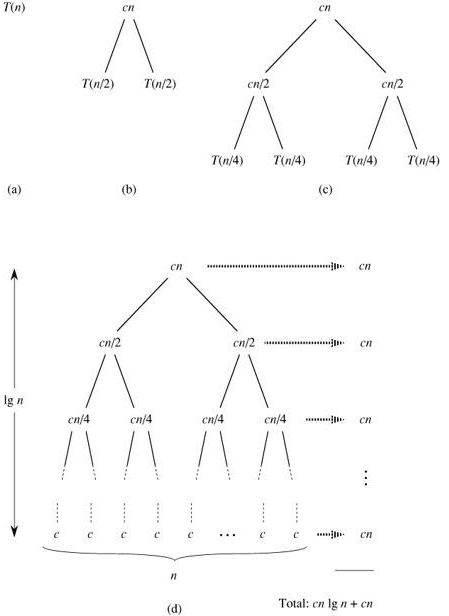
\includegraphics[scale = 0.7]{recursion_tree}\\
  \caption{Recursion tree example}\label{fig.compute.recursion_tree}
\end{figure}

为了便于计算,我们在这里设$\theta(1)=c$;
先把每一层的加起来,得到都是$cn$,然后再把所有层加起来,得到
$$T(n)=(lgn+1)cn=\Theta(nlgn)$$
So merge sort beats insertion sort.
$$ \theta(nlgn)<\theta(n^2) $$

\section{渐进符号,递归及解法}
\begin{definition}
\begin{figure}[htbp]
  \centering
  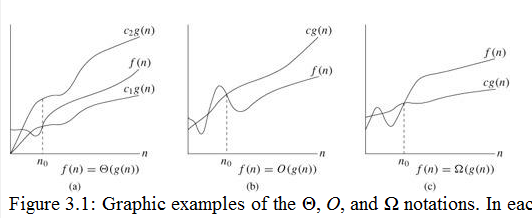
\includegraphics[scale = 0.7]{notation_asymptotical}\\
  \caption{Asymptotical notation}\label{fig.notation.asymptotical}
\end{figure}
\textbf{BIG O:上界 <=}\\
$O(g(n)) = \{f(n): $there exist positive constants $c$ and $n_0$ such that $0 \leq f(n) \leq cg(n)$ for all $n \geq n_0\}$\\
We say that $g(n)$ is an asymptotically upper bound for $f(n)$

\textbf{BIG $\Omega$下界 >=}\\
$\Omega(g(n)) = \{f(n): $there exist positive constants $c$ and $n_0$ such that $0 ≤ cg(n) ≤ f(n)$ for all $n ≥ n_0\}$\\
We say that $g(n)$ is an asymptotically lower bound for $f(n)$.

\textbf{BIG $\Theta$ =}\\
$\Theta(g(n)) = \{f(n) : $there exist positive constants $c_1, c_2$, and $n_0$ such that $0 ≤ c\lg n ≤ f(n) ≤ c_2g(n)$ for all $n ≥ n_0\}$\\
$$\Theta(g(n))=O(g(n)) \cap \Omega(g(n)) $$\\
We say that $g(n)$ is an asymptotically tight bound for $f(n)$.

The definition of $\Theta(g(n))$ requires that every member $f(n) ∈ \Theta(g(n))$ be asymptotically nonnegative, that is, that $f(n)$ be nonnegative whenever $n$ is sufficiently large.
\end{definition}

Ex:
$2n^2 + \Theta(n) = \Theta(n^2)$
for any function $f(n) ∈ \Theta(n)$, there is some function $g(n) ∈ \Theta(n^2)$ such that $2n^2 + f(n) = g(n)$ for all $n$. In other words, the right-hand side of an equation provides a coarser level of detail than the left-hand side.

o-notation
to denote an upper bound that is not asymptotically tight.\\
$o(g(n)) = \{f(n) : $for any positive constant $c > 0$, there exists a constant $n_0 > 0$ such that $0 ≤ f(n) < cg(n)$ for all $n ≥ n_0\}$\\
For example, $2n = o(n^2)$, but $2n^2 ≠ o(n^2)$

o-notation表示的是一种相差比较大的\\
in the o-notation, the function $f(n)$ becomes insignificant relative to $g(n)$ as $n$ approaches infinity; that is,
\end{document}
